\documentclass{article}
\usepackage[utf8]{inputenc}
\usepackage[frenchb]{babel}
\usepackage{tcolorbox}
\usepackage{tabularx}
\usepackage{array}
\usepackage{colortbl}
\tcbuselibrary{skins}
\usepackage[T1]{fontenc}



%------------ NICE TABS ----------%
\tcbset{note/.style={enhanced,fonttitle=\bfseries,fontupper=\normalsize\sffamily,
		colback=lime!20!white,colframe=lime!50!black}}

\tcbset{question/.style={enhanced,fonttitle=\bfseries,fontupper=\normalsize\sffamily,
		colback=teal!20!white,colframe=teal!50!black}}

\tcbset{attention/.style={enhanced,fonttitle=\bfseries,fontupper=\normalsize\sffamily,
		colback=red!20!white,colframe=red!50!black}}


%------------- MY ENVS --------%
\newcounter{note}[section]
\newenvironment{note}[1][]
{	
	
	\refstepcounter{note}
	
	
	
	\begin{center}
		\begin{tcolorbox}[note]
			\textbf{\textcolor{lime!30!black}{Note \arabic{section}.\arabic{note}}} :
			\begin{em}
			}
			{
			\end{em}
		\end{tcolorbox}	
	\end{center}
}



\newcounter{question}[section]
\newenvironment{question}[1][]
{	
	
	\refstepcounter{question}
	
	
	
	\begin{center}
		\begin{tcolorbox}[question]
			\textbf{\textcolor{teal}{Question \arabic{section}.\arabic{question}}} :
		}
		{
		\end{tcolorbox}	
	\end{center}
}


\newcounter{attention}[section]
\newenvironment{attention}[1][]
{	
	
	\refstepcounter{attention}
	
	
	
	\begin{center}
		\begin{tcolorbox}[attention]
			\textbf{\textcolor{red}{Attention \arabic{section}.\arabic{attention}}} :
			\begin{bf}
			}
			{
			\end{bf}
		\end{tcolorbox}	
	\end{center}
}

\author{Benjamin André\\Alexis Lecocq\\Arnaud Collin\\Waelkens Dimitri}
\title{Rapport de TP : CISCO}



\begin{document}

\maketitle

\section{Introduction}%rappel vite fait de l'énoncé et explication sommaire du rapport

\section{Description de votre Bunsiness Unit}

\section{Justification des choix liés à la configuration intra--domaine / inter-domaine (adressage, interfaces..)}

\section{Log des commandes utilisées sur vos routeurs Cisco}

R2\#show running-config
Building configuration...

Current configuration : 612 bytes

version 12.2
service timestamps debug uptime
service timestamps log uptime
no service password-encryption

hostname R2

memory-size iomem 30
ip subnet-zero

ip dhcp database VLAN2

ip dhcp pool VLAN2
   network 10.2.1.0 255.255.255.0
   dns-server 8.8.8.8
   default-router 10.2.1.1

interface Ethernet0/0
 ip address 10.2.0.2 255.255.255.252
 half-duplex

interface Ethernet0/1
 ip address 10.2.1.1 255.255.255.0
 half-duplex

ip classless
ip route 10.2.0.0 255.255.255.252 10.2.0.1
ip route 10.2.0.0 255.255.255.252 Ethernet0/0
ip http server

line con 0
line aux 0
line vty 0 4

end

\section{Problèmes rencontrés}

Tout dabord, nous avons eu un souci lors de la mise en place du service DHCP. Nous avons testés
plusieurs fois les commandes fournies dans l'énoncé mais sans succès.Nous avons dû regadrer dans 
la documentation de Cisco (disponible en ligne) afin de trouver une autre solution.

En testant les différentes solutions proposées, nous avons fini par remarquer que le routeur
ne reconnaissait pas certaines commandes. Nous avons donc supposé que le problème venait de celui-ci
et nous l'avons réinitialisé.

Après la réinitialisation du routeur, nous avons remis en place le service DHCP de façon similaire 
à la configuration effectuée à la base. Plus aucun souci constaté, le service fournissant des adresses
aux machines faisant la demande (effectué automatiquement lorsque celle-ci n'a pas d'adresse physique et se connecte à notre domaine).
\section{Erreurs connues dans votre configuration}

\section{Connexion entre différents groupes}

Certains liens devaient être administrés par différents groupes. Il a été nécessaire de les contacter pour connaître les conventions qu'ils utilisaient pour configurer les routers. Dès lors, nos routers ont été configuré de la sorte que ceux en bordure de notre réseau servent de passerelle vers les préfixes des autres groupes.

Des liens statiques vers leurs \emph{range} d'IP ont donc été établis.

\begin{question}
	Le résultat fut-il au rendez-vous ?
\end{question}

\noindent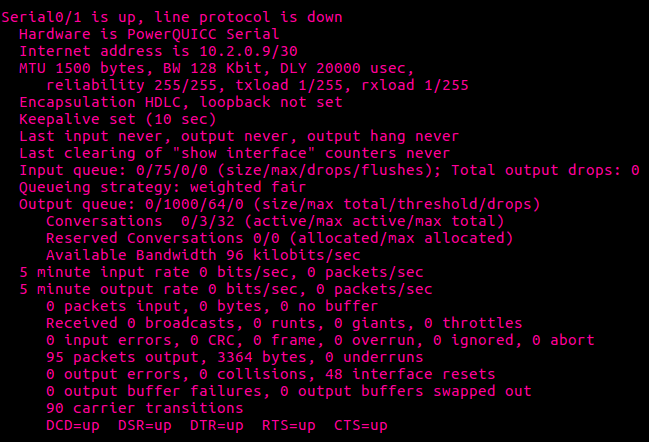
\includegraphics[width=\linewidth]{serialup}\\

Dans l'extrait de la console CISCO ci-dessus, on peut voir que notre interface seriel 0/1 est active, mais que le protocole ne l'est pas. Ceci s'explique dans ce cas-ci par le fait qu'il n'y avait aucune interface active à l'autre bout du câble.

Pouvoir s'y connecter aurait été une première étape vers le partage de routes, et donc le routage selon la topologie proposée dans l'énoncé.

\section{Conclusion}
Le routage est plus compliqué en pratique car il faut maîtriser un langage de configuration et des outils en plus de la théorie. C'est une phase de la conception d'un réseau à ne pas négliger. En effet, nous n'avons pas réussi à atteindre les objectifs dans le temps imparti pour ce TP.



\end{document}
